% ------------------------- 导言 ------------------------- %
\documentclass{article}
\usepackage[fontset=ubuntu]{ctex} % 用于解决中文问题
\usepackage{fancyhdr} % 用于自定义页眉与页脚
\usepackage[ 
    a4paper, % 每一页都是 a4 纸的大小
    textwidth=18cm, % 设置文本区域的宽度
    headheight=12mm, % 设置页眉的高度
]{geometry} % 用于设置页面布局
\usepackage{graphicx} % 用来插入图片
\usepackage{enumitem} % 用来调整列表缩进
\usepackage{colortbl} % 为表头添加背景色
\usepackage{xcolor} % 用来设置颜色
\usepackage{listings} % 用来插入代码
\usepackage{amsmath} % 额外的一些数学符号
% ------------------------- 变量 ------------------------- %
\newcommand{\titleText}{计算机程序理论与模型}
\newcommand{\subTitleText}{第 1 次作业}
\newcommand{\authorID}{12345678}
\newcommand{\authorName}{张三}
% ------------------------- 文字区域 ------------------------- %
\begin{document}
% -------------------- 颜色定义 -------------------- %
\definecolor{dkgreen}{rgb}{0,0.6,0}
\definecolor{gray}{rgb}{0.5,0.5,0.5}
\definecolor{mauve}{rgb}{0.58,0,0.82}
% -------------------- 页眉设置 -------------------- %
\pagestyle{fancy}
\fancyhf{} % 清除内置的页眉和页脚样式
\fancyhead[L]{\fontsize{4mm}{4.8mm}\selectfont\titleText:\subTitleText} % 设置页眉左侧
\fancyhead[R]{\fontsize{4mm}{4.8mm}\selectfont\authorID\authorName} % 设置页眉右侧
\fancyfoot[C]{\thepage}
\renewcommand{\headrule}{ % 重新设置页眉下方的水平线
    \vspace{-5mm} % 将页眉中的内容进行位置调整
    \hrulefill % 生成一个水平线
    \raisebox{-5mm}{
        \quad % 空格
        
\includegraphics[height=10mm]{logo/sysu_logo.png} % 学校 logo
        \quad
    }
    \hrulefill
}
% -------------------- 代码块设置 -------------------- %
\lstset{
    frame=tb,
    language=Python,
    aboveskip=3mm,
    belowskip=3mm,
    showstringspaces=false,
    columns=flexible,
    basicstyle={\small\ttfamily},
    numbers=none,
    numberstyle=\tiny\color{gray},
    keywordstyle=\color{blue},
    commentstyle=\color{dkgreen},
    stringstyle=\color{mauve},
    breaklines=true,
    breakatwhitespace=true,
    tabsize=3
}
% -------------------- 标题 -------------------- %
\title{
    \titleText \\
    \large \subTitleText
}
\author{\authorID\authorName}
\date{} % 清除时间,使其不要在标题中显示
\maketitle % 显示标题
\thispagestyle{fancy} % 在第一页也显示页眉
% -------------------- 正文 -------------------- %
\section{PySAT 求解 Refutation example 1 中的问题}
\subsection{Refutation example 1 中的问题介绍}

我们的知识库(Knowledge Base, KB)包含以下信息:

\begin{itemize}[leftmargin=2cm]
    \item FirstGrade
    \item FirstGrade $\to$ Child
    \item Child $\wedge$ Male $\to$ Boy
    \item Kindergarten $\to$ Child
    \item Child $\wedge$ Female $\to$ Girl
    \item Female
\end{itemize}

我们需要使用PySAT从KB推断出Girl,即证明KB $\models$ Girl。

\begin{table}[!htbp]
    \centering
    
    \begin{tabular}{|c|c|}
        \hline
        \rowcolor{gray!30} \textbf{Atom} & \textbf{Boolean Variable} \\
        \hline
        FirstGrade & $x_1$\\
        \hline
        Child & $x_2$\\
        \hline
        Male & $x_3$\\
        \hline
        Boy & $x_4$\\
        \hline
        Kindergarten & $x_5$\\
        \hline
        Female & $x_6$\\
        \hline
        Girl & $x_7$\\
        \hline
    \end{tabular}
    \caption{原子命题与布尔变量的对应关系}
    \label{tab:my_label}
\end{table}

\subsection{使用 PySAT 求解上述问题}

接下来我们通过将 PySAT 来求解上述问题。

\subsubsection{将问题转换为 SAT 问题}

为了求解上述问题,我们首先需要将原问题转换为 SAT 问题,换句话说,我们需要将“证明KB $\models$ Girl”转换为证明某个布尔公式不可满足,为了简化问题,我们先将各个原子命题(atom)转换为布尔变量$x_i$,KB 中的 7 个原子命题对应 7 个布尔变量,其中的对应关系如表1所示。

为了证明KB $\models$ Girl,即证明KB $\wedge$ $\neg$ Girl是不可满足的(unsatisfiable),我们可以将KB $\wedge$ $\neg$ Girl转换为公式(formula),该公式中的原子命题都通过表1转换为了对应的布尔变量,此时问题就转换为证明以下公式(1)是不可满足的。

\begin{equation}
    x_1 \wedge (x_1 \to x_2) \wedge (x_2 \wedge x_3 \to x_4) \wedge (x_5 \to x_2) \wedge (x_2 \wedge x_6 \to x_7) \wedge x_6 \wedge \neg x_7
\end{equation}

接下来,我们需要将公式(1)转换为 CNF 范式。

首先,我们将其中的条件语句转换为析取语句,即将$p \to q$转换为$\neg p \vee q$,对于公式(1)应用该转换规则之后即可得到公式(2)。

\begin{equation}
    x_1 \wedge (\neg x_1 \vee x_2) \wedge (\neg(x_2 \wedge x_3) \vee x_4) \wedge (\neg x_5 \vee x_2) \wedge (\neg(x_2 \wedge x_6) \vee x_7) \wedge x_6 \wedge \neg x_7
\end{equation}

接着再应用德摩根定律(De Morgan's Laws),将其中$\neg(x_2 \wedge x_3) \vee x_4$转换为$(\neg x_2 \vee \neg x_3) \vee x_4$,以及将$\neg(x_2 \wedge x_6) \vee x_7$转换为$(\neg x_2 \vee \neg x_6) \vee x_7$,接着将其中多余的括号去掉,即可得到公式(3)。公式(3)是一系列析取子句的合取,故公式(3)是 CNF 范式。

\begin{equation}
    x_1 \wedge (\neg x_1 \vee x_2) \wedge (\neg x_2 \vee \neg x_3 \vee x_4) \wedge (\neg x_5 \vee x_2) \wedge (\neg x_2 \vee \neg x_6 \vee x_7) \wedge x_6 \wedge \neg x_7
\end{equation}

此时原问题就转换为如何证明公式(3)不可满足,即原问题转换为了求解 SAT 问题。

\subsubsection{用 PySAT 求解上述 SAT 问题}

接下来我们将用 PySAT 来求解上述 SAT 问题,碍于篇幅,完整代码请看附录 A 或者附件,在这一小节我们只展示核心代码部分。

首先我们需要将之前得到的 CNF 范式输入到 PySAT 中,也就是将公式(3)输入到 PySAT 中。由于 PySAT 中使用自然数 $i$ 来表示布尔变量 $x_i$,故公式(3)可以按照下面的方式输入到 PySAT 中:

\begin{lstlisting}
# 输入 CNF 范式,其中 "1" 表示 "x1","2" 表示 "x2"
cnf = CNF(from_clauses=[
    [1], [-1, 2], [-2, -3, 4], [-5, 2], [-2, -6, 7], [6], [-7]
])
\end{lstlisting}

接下来利用 PySAT 中的 Solver 来判断该 CNF 范式是否可满足:

\begin{lstlisting}
# 使用 Solver 判断该 CNF 范式是否可满足
with Solver(bootstrap_with=cnf) as solver:
    # 输入该 CNF 范式是否可满足
    print('formula is', f'{"s" if solver.solve() else "uns"}atisfieable')
\end{lstlisting}

在命令行中运行上述 python 代码,即可得到图 1 中的结果,可以看到该 CNF 范式是不可满足的,即可得出 KB $\models$ Girl,证毕。

\begin{figure}[h]
    \centering
    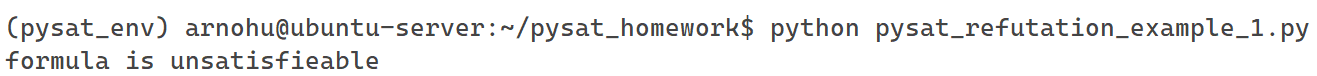
\includegraphics[width=1.0\textwidth]{figures/homework1_result.png}
    \caption{PySAT 求解公式(3) 是否可满足}
\end{figure}

\section{使用 PySAT 求解 N 皇后问题}

\subsection{N 皇后问题描述}

给定 $N$ 个皇后和一个 $N \times N$ 的棋盘,要求找到一种在该棋盘上放置 $N$ 个皇后的方法,使得每个皇后不能互相攻击彼此,即对于每个皇后 $i$ 来说,它的同一行,同一列,同一主次对角线都不会出现另一个皇后 $j$。

\subsection{将 N 皇后问题转换为 SAT 问题}

我们需要用 CNF 范式将 N 皇后问题表示出来。为了方便后续的讲解,我们用布尔变量$q_{i,j}$表示棋盘的第$i$行中的第$j$放置了一个皇后。

由于棋盘大小为$N \times N$,并且我们有 $N$ 个皇后,再加上同一行不能出现两个皇后,所以每一行必须有一个皇后存在。若我们想要表示第 $i$ 行必须有一个皇后存在,可以用$\bigvee_{j=0}^{N-1}p_{i,j}$来表示。那么“每一行必须有一个皇后存在”则可以用$\bigwedge_{i=0}^{N-1}\bigvee_{j=0}^{N-1}p_{i,j}$来表示。同理“每一列必须有一个皇后存在”可以用$\bigwedge_{j=0}^{N-1}\bigvee_{i=0}^{N-1}p_{i,j}$来表示。

接下来我们将皇后的各个互斥规则转换为公式。

对于第$i$行来说,不同列不能同时出现皇后,即$\bigwedge_{j=0}^{N-2}\bigwedge_{k=j+1}^{N-1}(\neg (p_{i,j} \wedge p_{i, k}))$,通过德摩根定律即可得到$\bigwedge_{j=0}^{N-2}\bigwedge_{k=j+1}^{N-1}(\neg p_{i,j} \vee \neg p_{i, k})$,故“每一行都不能同时有两个皇后”即为$\bigwedge_{i=0}^{N-1} \bigwedge_{j=0}^{N-2}\bigwedge_{k=j+1}^{N-1}(\neg p_{i,j} \vee \neg p_{i, k})$。

同理“每一列都不能同时有两个皇后”即为$\bigwedge_{i=0}^{N-1} \bigwedge_{j=0}^{N-2}\bigwedge_{k=j+1}^{N-1}(\neg p_{j,i} \vee \neg p_{k, i})$。

若第$i$行第$j$与第$k$行第$l$列在同一主对角线,那么一定有$i-k=j-l$,故“同一主对角线不能同时有两个皇后”即为$\bigwedge_{\substack{i,j,k,l=0 \\ i-k=j-l \\ i \neq k}}^{N-1} (\neg q_{i,j} \vee \neg q_{k,l})$。

同理“同一次对角线不能同时有两个皇后”即为$\bigwedge_{\substack{i,j,k,l=0 \\ i+j=k+l \\ i \neq k}}^{N-1} (\neg q_{i,j} \vee \neg q_{k,l})$。

综上,将 N 皇后转换为 CNF 范式即为以下 6 个公式的合取:

\begin{align}
&\bigwedge_{i=0}^{N-1} \left( \bigvee_{j=0}^{N-1} q_{i,j} \right) \\
&\bigwedge_{i=0}^{N-1} \left( \bigvee_{j=0}^{N-1} q_{j,i} \right) \\
&\bigwedge_{i=0}^{N-1} \bigwedge_{j=0}^{N-2} \bigwedge_{k=j+1}^{N-1} (\neg q_{i,j} \vee \neg q_{i,k}) \\
&\bigwedge_{j=0}^{N-1} \bigwedge_{i=0}^{N-2} \bigwedge_{k=i+1}^{N-1} (\neg q_{i,j} \vee \neg q_{k,j}) \\
&\bigwedge_{\substack{i,j,k,l=0 \\ i-k=j-l \\ i \neq k}}^{N-1} (\neg q_{i,j} \vee \neg q_{k,l}) \\
&\bigwedge_{\substack{i,j,k,l=0 \\ i+j=k+l \\ i \neq k}}^{N-1} (\neg q_{i,j} \vee \neg q_{k,l})
\end{align}

此时解决 N 皇后问题就转换为求解 SAT 问题。

\subsection{使用 PySAT 求解上述 SAT 问题}

碍于篇幅,这里只展示部分核心代码,完整代码请看附录 B 或者附件。在 PySAT 中自然数 $i$ 代表着布尔变量 $x_i$,而我们在 2.2 中的布尔变量都是 $p_{i,j}$ 的格式,故我们需要一个辅助函数来将$p_{i,j}$转换成$x_i$,换言之就是输入两个自然数$i$和$j$,然后得到新的自然数作为布尔变量的下标。该辅助函数如下:

\begin{lstlisting}
def varnum(i, j):
    # n 为 N 皇后问题的参数 N
    return n * i + j + 1
\end{lstlisting}

接下来我们要初始化一个空的 CNF 范式,然后依次将公式(4)~(9)填充进去,初始化 CNF 范式如下所示:

\begin{lstlisting}
formula = CNF()
\end{lstlisting}

接下来我们要往 formula 中填充公式(4)与公式(6),这两个公式能够确保同一行不出现两个皇后,且至少保证棋盘上有 N 个皇后,填充的过程如下:

\begin{lstlisting}
# 确保每行只有一个皇后,且保证棋盘中有 N 个皇后
for i in range(n):
    # 对应公式 (4)
    formula.append([varnum(i, j) for j in range(n)])
    for j in range(n-1):
        for k in range(j+1, n):
            # 对应公式 (6)
            formula.append([-varnum(i, j), -varnum(i, k)])
\end{lstlisting}

同理,我们可以用类似的方式来填充公式(5)和公式(7),这两个公式能够确保同一列不出现两个皇后,且保证棋盘上有 N 个皇后,填充的过程如下:

\begin{lstlisting}
# 确保每列只有一个皇后,且保证棋盘中有 N 个皇后
for j in range(n):
    # 对应公式 (5)
    formula.append([varnum(i, j) for i in range(n)])
    for i in range(n-1):
        for k in range(i+1, n):
            # 对应公式 (7)
            formula.append([-varnum(i, j), -varnum(k, j)])
\end{lstlisting}

而公式(8)和公式(9)分别对应着主对角线最多只能有一个皇后和次对角线最多只能有一个皇后,我们可以直接公式写出以下代码:

\begin{lstlisting}
# 确保没有两个皇后在同一主对角线,同时确保没有两个皇后在同一次对角线
for i in range(n):
    for j in range(n):
        for k in range(n):
            for l in range(n):
                if i != k and i - k == j - l:
                    # 对应公式 (8)
                    formula.append([-varnum(i, j), -varnum(k, l)])
                if i != k and i + j == k + l:
                    # 对应公式 (9)
                    formula.append([-varnum(i, j), -varnum(k, l)])
\end{lstlisting}

至此,我们已经将 N 皇后问题对应的 CNF 范式输入进了 formula 变量中,接下来使用 SAT 求解器进行求解即可,若求解出某个变量为正数,则表示那个变量对应的位置可以放一个皇后,为了对结果进行可视化,可以放皇后的地方用 "Q" 来表示,而不可以放皇后的地方则用 "." 表示,如下所示:

\begin{lstlisting}
with Solver(bootstrap_with=formula) as solver:
    if solver.solve():
        model = solver.get_model()
        board = [['.' for _ in range(n)] for _ in range(n)]
        for val in model:
            if val > 0:  # 检查正的变量值,正的变量表示当前位置可以放一个皇后
                i = (val - 1) // n # 从 val 中解析出行号
                j = (val - 1) % n  # 从 val 解析出列好
                board[i][j] = 'Q'
        return board
    else:
        return None
\end{lstlisting}

当我们输入 N = 8 的时候,结果如图 2 所示,当我们输入 N = 10 的时候,结果如图 3 所示,可以看出我们的求解的结果是正确的。

\begin{figure}[h]
    \centering
    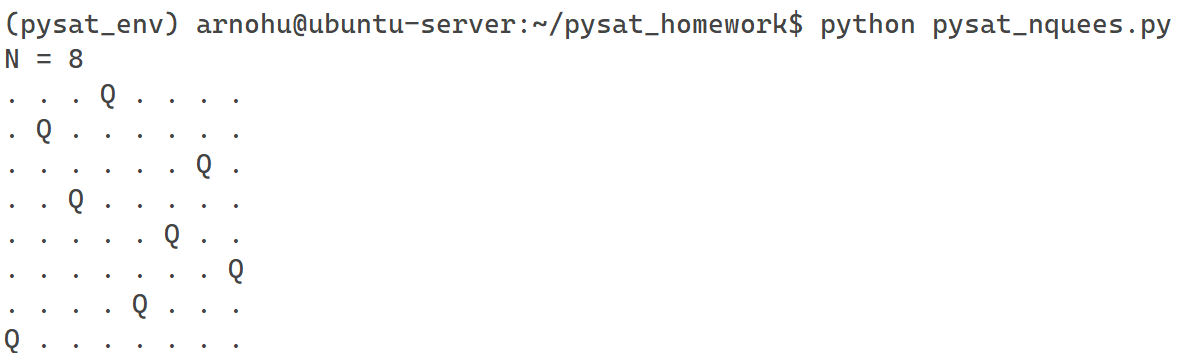
\includegraphics[width=1.0\textwidth]{figures/nqueens_8.png}
    \caption{PySAT 求解 8 皇后问题}
\end{figure}

\begin{figure}[h]
    \centering
    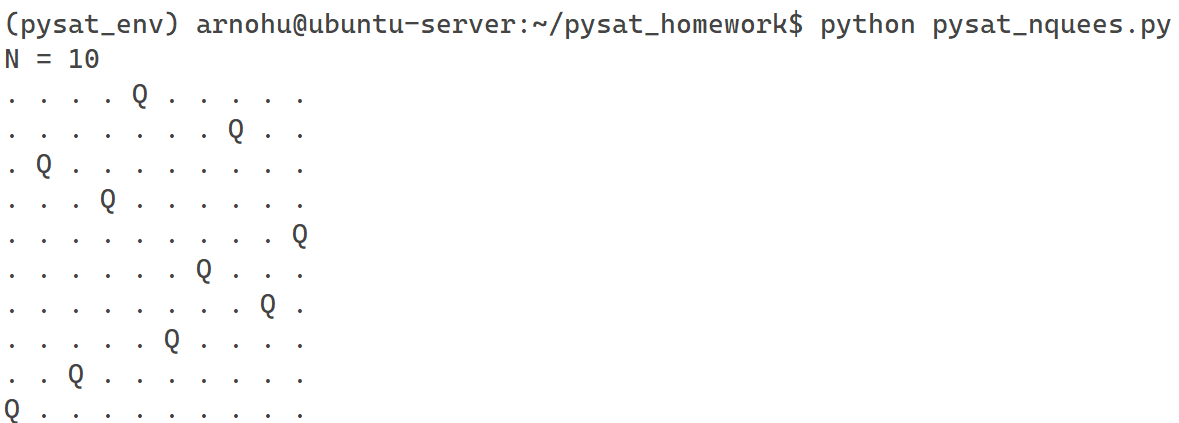
\includegraphics[width=1.0\textwidth]{figures/nqueens_10.png}
    \caption{PySAT 求解 10 皇后问题}
\end{figure}

\end{document}